\section{Processing of a Single Subject-Verb Dependency in NLMs}
In the classic number agreement task (NA-task), subjects are presented with the beginning of a sentence (aka, `preamble') that contains a long-range subject-verb relation, such as: ``The keys to the cabinet\ldots'', and are asked to predict the verb to follow (e.g., ``are''). Human subjects make more agreement errors (e.g., continuing the preamble  above with ``is'' instead of ``are'') when the intervening noun (aka, `attractor') has a different grammatical number than the main subject (as in the preamble above, with plural subject ``keys'' and singular attractor ``cabinet'') . Behavioral measures collected during agreement tasks, such as error-rates, vary as a function of the syntactic environment of the long-range dependency. This has provided rich data to test hypotheses regarding online syntactic processing in humans \citep[e.g., ][]{franck2002subject, franck2006agreement, franck2007syntactic}.

Starting with the influential work of \citet{Linzen:etal:2016}, a growing
literature \citep[e.g.,][]{Gulordava:etal:2018, Bernardy:Lappin:2017,
  Giulianelli:etal:2018, Kuncoro:etal:2018a,Linzen:Leonard:2018,jumelet2019analysing} has
tested NLMs on the NA-task at the behavioural level, showing that these models have performance
and error patterns partially resembling those of humans.
More recently, we investigated the underlying neural mechanism of an
English NLM during the processing of a long-range dependency
\citep{lakretz2019emergence}. We identified a neural circuit in the
network that encodes and carries grammatical number across long-range
dependencies, showing also that processing in NLMs is sensitive to the
structure of the subject-verb dependency. In the next section we
describe the main findings of our previous study, followed by a replication of them in a NLM trained on Italian. 

\YL{Add something of the sort - readers that are familiar with previous findings can also safely continue to the next section.}


\subsection{Agreement in the English NLM}

\subsubsection{The Noun-PP Number-Agreement Task}
The main NA-task used by \citet{lakretz2019emergence} contained sentences with a subject-verb dependency separated by a prepositional phrase (e.g., ``The \textbf{boy} near the car \textbf{smiles}''), referred to as the `Noun-PP' task. This task comprises four conditions, which correspond to the four possible assignments of grammatical number to the main subject and attractor (SS, SP, PS and PP; S-singular, P-plural). The NLM was presented with preambles of sentences from this task, and predictions of the model of the next word were then extracted, from which error-rates were computed (Methods). 

\subsubsection{Long-Range Number Units}
Having verified that the network could predict the correct number with high accuracy, \citet{lakretz2019emergence} tested whether there were units in the network that were crucial to carry grammatical number across long-range dependencies.  To identify such units, \citet{lakretz2019emergence} conducted an ablation study, by removing a unit of the NLM at a time, and re-evaluating its performance on the Noun-PP NA-task. The ablation revealed that two (out of 1300) units in the network each caused a reduction in agreement performance towards chance level when ablated. One of these units only affected performance when the main subject of the sentence was singular, and was therefore called the `singular unit'. The other unit had an effect with plural subjects only, hence, the `plural unit'. 
No other unit had a comparable effect on network performance when ablated. A visualization of state dynamics of the singular and plural units confirmed their role in encoding and carrying through grammatical number across long-range dependency, robustly also in the presence of an attractor \citep[figure 1 in][]{lakretz2019emergence}.

\subsubsection{Syntax Units}
Since the activity of the long-range number units follow the structure of the syntactic long-range dependency, \citet{lakretz2019emergence} tested whether other units in the network encode syntactic information and inform the long-range number units about when to store and release number information in their encoding. Several units were found to have activity that is predictive about transient syntactic properties of the sentence. In particular, the activity of one of these `syntax' units followed the structure of the main subject-verb dependency, consistently across various sentence constructions \citep[figure 3 in][]{lakretz2019emergence}. 

\subsubsection{Short-Range Number Units}
\citet{lakretz2019emergence} further found that grammatical number information was also encoded
by other units in the network. Number information can still be
decoded from network activity even when the long-range number units
are removed. However, number information encoded in these other units is short-lived. Whenever new grammatical number information is
introduced (e.g., upon encountering a noun or a verb), activity in
these units abruptly switches to represent this last encountered
number. These `Short-Range Number Units' can therefore only support number-agreement dependencies that do not
enfold attractors (e.g., "The \textbf{boy} gracefully
\textbf{smiles}"). The presence of short-range number units explain why ablating the long-range circuit only affects agreement in long-distance dependencies.


\subsection{Agreement in the Italian NLM}
The choice to focus on Italian instead of English is based on two main reasons reasons. First, we found that the Italian NLM made available by \citet{Gulordava:etal:2018} achieves better performance than the English NLM on nested construction, which are computationally more demanding compared to sentences in the Noun-PP NA-task explored in \citet{lakretz2019emergence}. This might be explained by that Italian is morpho-syntactically richer than English. Second, in English, the plural is identical to the unmarked form of the verb, which can occur as infinitive, in first and second person, and often as a noun. This makes the occurrence statistics unbalanced, in favor of plural. \footnote{\citet{Gulordava:etal:2018} made available models in English, Italian, Hebrew and Russian, which were optimized by conducting a grid search, and became since a subject of research in several subsequent studies \citep{Giulianelli:etal:2018, jumelet2019analysing, wilcox2018rnn, futrell2019neural}. We therefore did not consider repeating the optimization process in these or other languages and used the same set of hypterparameters reported by this study when training additional NLMs (methods). Given the above considerations, Hebrew and Italian might have been also good alternative for the purpose of this study. \YL{not sure if all this is really needed}.}

To test whether the Italian NLM has developed an agreement mechanism similar to the model trained on English, we followed the same steps described in the previous section - an ablation study, visualization of unit dynamics and a connectivity analysis.

\subsubsection{Ablation Results Reveal a Long-Range Number Unit} To identify unit(s) that encode grammatical number for long-range dependencies, we conducted an ablation study on the Italian model made available by \citet{Gulordava:etal:2018}, following the steps described above, using an Italian noun-PP NA-task (Methods). We found that the ablation of one unit from the second layer of the network, unit 815, led to a significant reduction in performance in both incongruent conditions (figure S1).\footnote{We repeated the ablation experiment also with another 19 NLMs that we trained on the same corpus and found that most models showed a significant reduction in performance after unit ablation, for only a few units, with some models showing a significant effect on the SP or PS condition only, and others on both (figure S2).}

\subsubsection{Dynamics of the Number Unit Show Robustness to Attractors} 
To confirm that unit 815 is a long-range number unit, we visualized the dynamics of the unit during the processing of the long-range dependency, by extracting its activations during the processing of all sentences in the noun-PP NA-task. Figure \ref{fig:nounpp}A describes the resulting average cell-state activations. It shows that number information is robustly encoded throughout the subject-verb dependency, also in the presence of an attractor (dashed lines). Furthermore, the dynamics of unit 815 show that it encodes both singular and plural number, using negative and positive cell activations, respectively.

\subsubsection{Efferent Weights of the Number Unit are Clustered with Respect to Number}
Finally, we extracted the efferent weights of unit 815, which project onto the output layer. Figure S2A shows that unit 815 deferentially affects unit activations in the output layer, depending on whether they represent singular or plural forms of the verb. This is consistent with its role as a number unit. In what follows, we refer to unit 815 as the long-range `Number Unit'.

\subsubsection{Long-Range Gender Units are Also Found in the Network }
Agreement in Italian can also occur with respect to gender, for instance, in sentences containing predicative adjectives: ``\textbf{Il bambino} accanto al madre \`{e} \textbf{bello}'' (``The boy near the mother is pretty''), in which the subject and adjective agree with respect to both number and gender. We therefore hypothesized that there should also exist long-range `gender' units in the network, with dynamics that are robust to possible attractors (e.g., to "madre" above, which is feminine). Using an NA-task with adjective phrases and repeating the ablation study (Methods), we found that one unit dramatically reduced the performance of the NLM when ablated, and its inner-state dynamics showed robust encoding across the subject-adjective dependency (Figure \ref{fig:nounpp}A), also in the presence of attractors (dashed lines). Connectivity analysis further confirmed that the efferent weights of the long-range `gender' unit were clustered with respect to whether they project to masculine or feminine adjective words in the output layer (figure S2B).

\vspace{10pt}
In sum, these results extend previous findings to another language and another grammatical feature. Similarly to English, only a few long-range number units emerged in the Italian NLMs during training, in the majority of the cases. The NLM has developed a similar encoding scheme for both grammatical number and gender, independently. Taken together, this shows that sparse long-range feature units consistently emerge in NLMs.

\YL{(we may need to specify that our lexicon included only biological gender, or repeat the experiments with also inanimates.)}. 

\begin{figure}
    \centering
    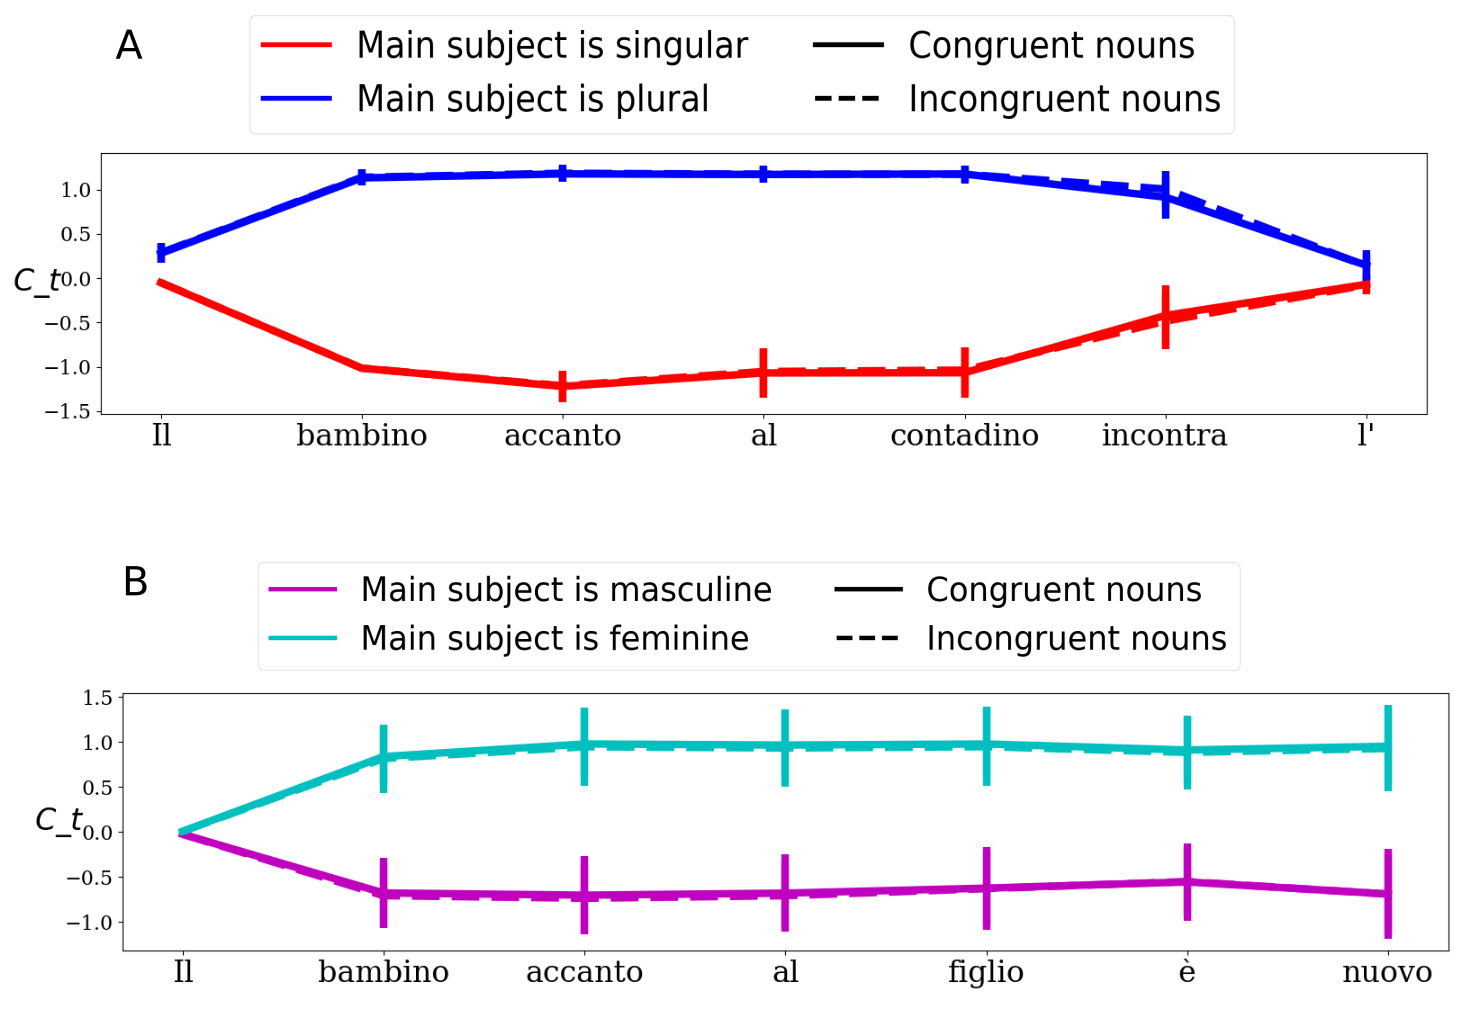
\includegraphics[width=\textwidth]{figures/model_activations_nounpp.png}
    \caption{\textbf{Cell activity of the number unit (panel A) and gender unit (panel B) during the processing of a single long-range dependency across a prepositional phrase:} four conditions are presented, corresponding to whether the main subject of the sentence is singular (red curves) or plural (blue), and to whether the main subject (`bambino') and the intervening noun (`contadino') have the same (congruent) or opposite number (incongruent)}
    \label{fig:nounpp}
\end{figure} 
